% Introduction

\section{Scope of this study}

A growing number of Australian firms are turning towards open innovation as a competitive strategy. Not only does this enable them to access external knowledge resources, it also allows them to profit from internally developed knowledge by making it available to other firms \citep{chesbrough2003open}. However, open innovation is not without its management challenges. Relative differences in absorptive capacity can undermine efforts to transfer knowledge across organisational boundaries \citep{nooteboom2000learning}. Though tacit knowledge is important for reducing the cognitive distance between open innovation partners \citep{nonaka1994dynamic,carlile2004transferring,collins2006leveraging,lichtenthaler2016absorptive}, not much is known about the social mechanisms underpinning tacit knowledge exchange in open innovation. This study attempts to fill this gap in understanding by examining tacit knowledge sharing in three open innovation projects and how such knowledge can help overcome relative differences in absorptive capacity. Particular attention is given to how people are motivated to share tacit knowledge and what different patterns of tacit knowledge brokerage reveal about trust and power relations in open innovation partnerships. \medskip

\section{Background}

\subsection{Need to innovate}

Innovation can be defined as the process of implementing new ideas to create value for an organisation \citep{schumpeter1950capitalism}. As long an idea is perceived as new by all those involved, it is an innovation even though it may appear to others as nothing more than an imitation of something that already exists elsewhere \citep{van1986central}. Failure to innovate places a firm’s ability to survive and prosper at grave risk \citep{bessant2005managing}. \medskip

Though Australia performs particularly well with respect to knowledge creation, it fares poorly when it comes to transforming knowledge into new-to-market innovations. Much of Australia's prosperity stems from its natural advantages in agriculture and mining \citep{leung2016view}. Unfortunately, this has suppressed the need to innovate, resulting in an under-performing national innovation system. Australia lags other Organisation for Economic Cooperation and Development (OECD) countries in terms of university-industry collaborations and number of researchers employed in the business sector \citep{dodgson2011changing,pettigrew2012australia,leung2016view}. Shrinking demand for it's mineral resources and increased regional competition means that Australia no longer can rely on its natural advantages for economic prosperity. Australian firms need to become better at innovation to compete in an increasingly borderless and fast-paced economy. \medskip

\subsection{Trend towards open innovation}

According to the resource-based view of the firm, competitive advantage stems from the application of tangible and intangible resources available to the firm \citep{wernerfelt1984resource,peteraf1993cornerstones}. Sustained competitive advantage can be achieved if these resources are valuable, rare, inimitable, and non-substitutable \citep{barney1991firm}. The knowledge-based view of the firm considers knowledge to be the most valuable resource of a firm \citep{grant1996toward}. Flowing from the knowledge-based view is the relational view of the firm, which suggests a firm's critical resources may reside be embedded in inferiirm resources and routines.

focuses on the social structures, routines, and processes for knowledge exchange \citep{grant1995knowledge,dyer1998relational,nahapiet1998social,tsai1998social}.  The relational view implies competitive advantage stems from the reach and richness of a firm's knowledge network and mechanisms for , the richness of knowledge embedded in the knowledge network, and the ability of the firm to access or channel knowledge across organisational boundaries \citep{gulati2011networks}. A firm's dynamic capability refers to its \enquote{ability to integrate, build, and reconfigure internal and external competences to address rapidly changing environments} \citep{teece2007explicating}. \medskip

Firms across the world are finding it is becoming harder to compete in the knowledge-based economy\footnote{The term \enquote{knowledge-based economy} refers to the increasing role of knowledge and technology in economic growth \citep{oecd1996knowledge}.}. Much of this can be attributed to the ever-increasing technical complexity of products, processes, and services that demand levels of knowledge beyond what most firms possess or can develop in a market-relevant time-frame. Consequently, many firms are turning towards open innovation as a competitive strategy \citep{enkel2009open,bessant2013innovation,stanko2017under}. Open innovation may be defined as a distributed innovation process based on carefully managed knowledge flows across firm boundaries, using mechanisms as per the firm's business model\footnote{The term \enquote{business model} refers to the design or architecture of the value creation, delivery, and capture mechanisms of a firm \citep{teece2010business}.}. The business model driving open innovation operationalises the relational view of competitive advantage by explicating the mechanisms used to create and capture value from inter-firm knowledge exchanges \citep{durst2013success,chesbrough2017future}. \medskip

Key benefits of open innovation include early access to new technology, sharing of risk, reduced costs of development, better customer acceptance of products or services, and enhanced ability to continuously innovate \citep{ye2013exploring}. Because distributed innovation processes are hard to observe and thus imitate, open innovation is also a useful strategy for sustaining competitive advantage \citep{barney1991firm,lichtenthaler2011open}. \medskip

\subsection{Open innovation processes}

Open innovation can be described in terms of inbound, outbound and coupled innovation processes \citep{gassmann2004towards}. Inbound open innovation enriches a firm’s knowledge base through integrating suppliers, customers and other external actors \citep{xu2013inbound} whereas outbound open innovation refers to the commercial exploitation of knowledge developed in-house \citep{de2016knowledge}. \emph{Coupled open innovation} focuses on strategic partnerships that encompass both inbound and outbound innovation processes \citep{spithoven2013open}. Figure \ref{fig:oi_process} illustrates how these processes may work in practice. \medskip

\begin{figure}
	\centering
	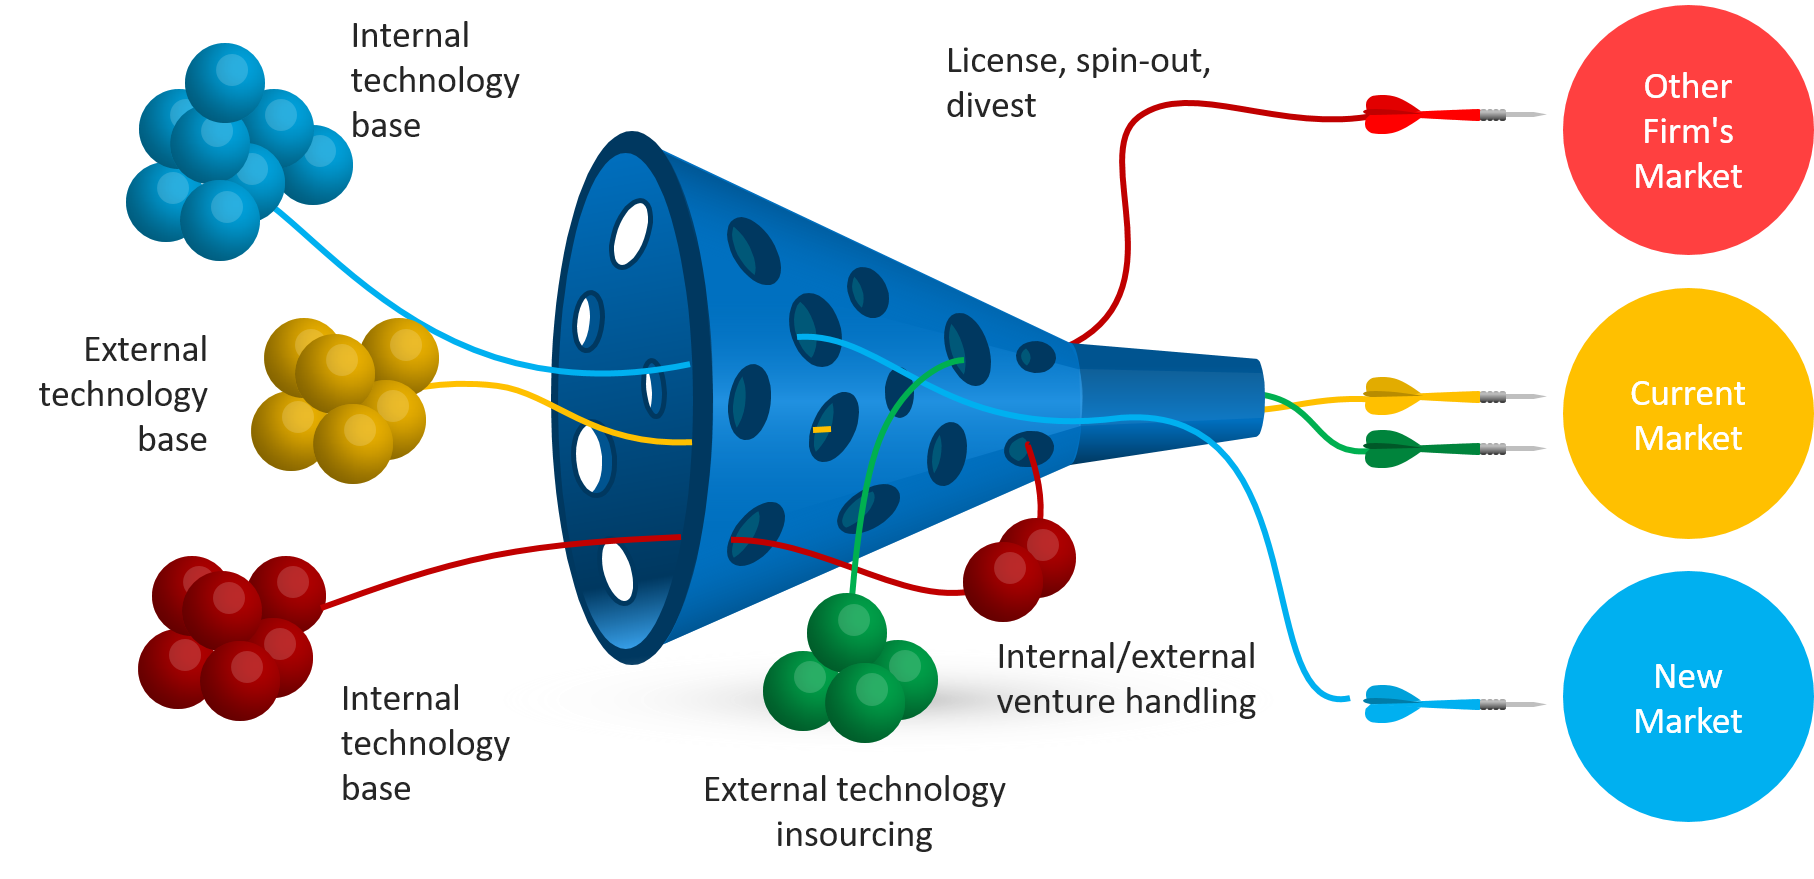
\includegraphics[width=0.9\linewidth]{oi_process_2}
	\caption{Open innovation processes \citep{chesbrough2004open}. Image from SlideModel\texttrademark.}.
	\label{fig:oi_process}
\end{figure}

The locus of control is different for each process. With inbound open innovation, the firm receiving new external knowledge controls the innovation process. This is not the case with outbound open innovation, where the locus of control is external to the firm that is providing knowledge. With coupled open innovation, partners jointly control the innovation process \citep{gassmann2004towards}. Different capabilities are needed for inbound, outbound, and coupled open innovation. Firms pursuing inbound open innovation need \enquote{absorptive capacity} to make sense of, and exploit, new external knowledge  \citep{vanhaverbeke2007connecting}. Firms wishing to exploit their internally developed knowledge through outbound open innovation require \enquote{desorptive capacity} to identify and act on knowledge transfer opportunities. This includes having appropriate mechanisms for managing and leveraging intellectual property \citep{lichtenthaler2010technology,chesbrough2012open}. The capacity to develop and maintain strong and productive inter-organisational networks is particularly important\citep{gassmann2004towards,chesbrough2012open}. Managers of open innovation projects need to ensure firms have sufficient dynamic capability to tackle inbound, outbound, and coupled open innovation. \medskip

\subsection{Challenges of open innovation}

Despite its many potential benefits, open innovation presents considerable management challenges. Three challenges stand out as particularly worthy of attention, namely dealing with relative differences in absorptive capacity \citep{vanhaverbeke2007connecting,robertson2012managing}, mobilising tacit knowledge \citep{wallin2010organizing,bogers2011open}, and brokering productive inter-organisational relationships \citep{fleming2007brokerage,gassmann2010future,whelan2011creating}. \medskip

\subsubsection{Relative differences in absorptive capacity}

Firms need absorptive capacity to make sense of new external knowledge and allow them to capture value from open innovation processes \citep{vanhaverbeke2007connecting,zobel2016benefiting}. The term \enquote{absorptive capacity} refers to the \enquote{ability of a firm to recognise the value of new, external information, assimilate it, and apply it to commercial ends} \citep{cohen1990absorptive}. Overcoming relative differences in absorptive capacity between partner firms is particularly challenging \citep{zobel2016benefiting}. Relative differences in absorptive capacity can impede the flow of knowledge across organisational boundaries, contribute to power imbalances, and undermine alliance performance, all of which can result in sub-optimal open innovation outcomes \citep{lane1998relative,vanhaverbeke2007connecting}.  \medskip

Absorptive capacity includes the capability to acquire and assimilate new external knowledge, referred to as \enquote{potential absorptive capacity}, and the capability to transform and exploit new external knowledge, referred to as \enquote{realised absorptive capacity} \citep{zahra2002absorptive}. Acquiring and assimilating new external knowledge is not sufficient by itself. Newly acquired knowledge has to be put to productive use to be truly valuable \citep{zobel2016benefiting}. The efficiency at which a firm can convert new acquired knowledge into valuable innovations can be expressed as the ratio of potential versus realised absorptive capacity \citep{zahra2002absorptive}. \medskip

Past studies of absorptive capacity emphasise the importance of prior knowledge possessed by individuals and groups \citep[e.g.][]{cohen1990absorptive,todorova2007absorptive,lichtenthaler2009absorptive}. Much of this prior knowledge is tacit in nature, embodied in the minds and actions of people \citep{lichtenthaler2016absorptive}. Tacit knowledge is associated with terms such as \enquote{intuition}, \enquote{skill}, \enquote{know-how}, and \enquote{expertise} used to describe knowledge that refers to an ability to perform work \citep{horvath2000working,mcadam2007exploring}. The most common application of tacit knowledge is problem-solving \citep{leonard1998role}. People with expertise borne from experience not only are able to recognise the situation they find themselves in, but also know which actions might be appropriate for dealing with it \citep{simon1971human}. Tacit knowledge can also used to re-frame problems or anticipate outcomes in intuitive ways \citep{leonard1998role}. Whereas explicit knowledge is revealed by its communication, tacit knowledge is revealed through its application and acquired through practice \citep{grant1996toward}. Without tacit knowledge, explicit knowledge quickly loses its meaning \citep{nonaka1994dynamic,seidler2008use}. Thus, tacit knowledge plays a key role in reducing cognitive distance between open innovation partners \citep{nooteboom2007optimal,goffin2010managing,szulanski2016overcoming}.  \medskip 
 
\subsubsection{Mobilising tacit knowledge}

Not only can tacit knowledge help reduce the cognitive distance between open innovation partners, it also guides the thinking that produces novel ideas \citep{leonard1998role,amar2008descriptive}. Mobilising tacit knowledge is particularly challenging because people are either unaware of the tacit dimension of their knowledge, or are unable to express what they know \citep{polanyi1966tacit,leonard1998role}. Moreover, many firms do not appreciate the diversity of their knowledge resource and lack processes to unlock the potential value of tacit knowledge embodied in the minds and actions of employees \citep{nonaka1994dynamic,horvath2000working}. Getting people to share their tacit knowledge is not something that can be mandated - it happens through volition or free will \citep{polanyi1966tacit}. Employees are inclined to hoard their knowledge to maintain some form of personal advantage \citep{eraut2000non,riege2005three,milne2007motivation}. People are unlikely to disclose their personal knowledge if this makes them feel more vulnerable \citep{levin2004strength}. Trust is an important prerequisite for tacit knowledge sharing \citep{kucharska2016trust}. \medskip

Adding to the challenge is the notion that tacit knowledge is not transferred but rather interpreted within a specific context \citep{nonaka1995knowledge,duguid2005art,marabelli2014knowing}. Face-to-face social interaction is key because it allows immediate feedback to check understanding and correct any misinterpretations \citep{koskinen2003tacit}. While advances in information technology (e.g. e-mail, instant messaging, collaborative web sites, video-conferencing) have made it easier for distributed team members to communicate with each other, much of this technology is not well-suited for tacit knowledge exchange and immediate feedback. This may negatively impact knowledge sharing and idea generation in open innovation \citep{johannessen2001mismanagement}. \medskip

% individual vs. group 
% emergence 
% dynamic capabilities
% complexity

\subsubsection{Brokering productive relationships} % fleming, whelan, gassman

Boundary spanners play a key role in open innovation as they promote cooperation and coordinated actions necessary to integrate and exploit diverse sources of knowledge \citep{fleming2007brokerage}. They broker new relations that extend or widen existing inter-organisational networks \citep{granovetter1973strength}. More importantly, boundary spanners facilitate the translation and integration of unfamiliar and distant knowledge i.e. help strengthen absorptive capacity \citep{tushman1981boundary,allen1984managing,fleming2007brokerage,meyer2010rise,tortoriello2010activating}. \medskip 

Management efforts to create or widen existing inter-organisational networks may be frustrated by people reluctant to form new ties, facilitate third-party ties, or otherwise change their existing networks \citep{davis2010agency}. Negative attitudes such as \enquote{not-invented-here} and \enquote{not-shared-here} (also referred to as \enquote{not-sold-here}) syndromes can also undermine efforts to develop and maintain strong and productive inter-organisational networks in open innovation \citep{lichtenthaler2006attitudes,lichtenthaler2011your,de2014neither,podmetina2015skills,chesbrough2017future}. Not-invented-here syndrome refers to resistance within a firm against externally developed knowledge \citep{katz1982investigating,hussinger2011search,antons2015opening}. Not-shared-here syndrome is a negative attitude towards external exploitation of internally developed knowledge \citep{chesbrough2003open,lichtenthaler2006attitudes,de2014neither}. Determining ways to overcome negative attitudes towards knowledge sharing, especially tacit knowledge sharing, is essential to allow the formation of new productive relationships that enable knowledge to be recombined in unique and valuable ways \citep{uzzi1997social,nahapiet1998social,obstfeld2005social,lane2006reification,davis2010agency,meyer2010rise}. \medskip

% fleming, maurer...
% shifting perspectives - educating people to pattern differently

\section{Research opportunity}

Knowledge networks represent collections of individuals and teams who come together across organisational, spatial and disciplinary boundaries to create, share or apply a body of knowledge \citep{pugh2013designing}. The business model underpinning open innovation, explains how value is generated from inter-organisational knowledge networks \citep{chiaroni2010unravelling}. As explained earlier, tacit knowledge plays a key role in translating knowledge i.e. it helps reduce the cognitive distance between senders and receivers of knowledge \citep{seidler2008use}. The extent to which tacit knowledge helps bridge cognitive gaps is poorly understood. Tacit knowledge has a significant influence on a firm's absorptive and innovative capacity, and warrants much more attention than it has received so far. Absorptive capacity may be construed as an emergent property of knowledge exchange networks \citep{tortoriello2015social}. We can use social network analysis to assess the role of tacit knowledge in open innovation and what this means in terms of absorptive capacity. \medskip

\subsection{Exploring motivational factors}

Tacit knowledge requires significantly more effort than explicit knowledge to communicate. People need to be sufficiently motivated to seek out and share tacit knowledge \citep{leonard1998role}. Past studies show a significant and positive relation between an individual's level of intrinsic motivation and the amount of tacit knowledge they share  \citep[e.g.][]{osterloh2000motivation,kaser2001knowledge,smith2001role}. Intrinsic motivation is about engaging in activity because it is enjoyable or personally meaningful \citep{ryan2000intrinsic}. Although these studies highlight the importance of personal motivation, the psycho-social processes underpinning tacit knowledge sharing and how this impacts open innovation are not well understood. This indicates a need to investigate how personal motivation shapes the development of knowledge sharing relations. \medskip

\subsection{Unpacking power-relations} 

Though it is often stated that \enquote{knowledge is power}, little attention has been  to power and power-relations in the knowledge management literature \citep{heizmann2015power}. The current power literature is dominated by two contrasting views of power, namely \enquote{power as domination}, also referred to as \enquote{power-over}, and \enquote{power as empowerment}, often characterised as \enquote{power-to} \citep{haugaard2012rethinking}. Sharing tacit knowledge is about empowering others so they can perform work more independently and confidently \citep{bordum2002tacit,lin2007share}. \medskip

The network perspective treats power as inherently relational \citep{ibarra1993network}. How an actor is embedded in a social network either imposes constraints on the actor or presents them with opportunities \citep{burt1992structural,simpson2011network}. Actors with fewer constraints and more opportunities occupy favourable structural positions. Being in a favoured position means that an actor may extract better bargains in exchanges, have greater influence, and be a focus for deference and attention from those in less favoured positions \citep{burt1992structural,hanneman2005introduction,simpson2011network}. \medskip

Actors in knowledge networks serve both as keepers of knowledge and as agents that seek out, communicate, and create knowledge \citep{phelps2012knowledge}. One can assess how actors exercise power by examining patterns of brokerage in knowledge sharing networks. Brokerage may be defined as the \enquote{behaviour by which an actor influences, manages, or facilitates interactions between other actors} \citep{obstfeld2014brokerage}. This definition allows brokerage to be seen in terms of \enquote{power-over} and \enquote{power-to}. \medskip
 
\section{Study objectives}

This study explores tacit knowledge sharing in three open innovation partnerships. Attention is focused on how people are motivated to share tacit knowledge and what patterns of social interaction tell us about tacit knowledge sharing processes in open innovation. The study also examines the organisational context in which tacit knowledge sharing takes place. Four research questions are addressed in this study: \medskip

\begin{description}
    \begin{enumerate}
        \item To what extent does the level and type of personal motivation predict tacit knowledge sharing in open innovation partnerships?
	    \item What does the configuration of tacit knowledge networks reveal about power-relations in open innovation partnerships?
	    \item What is the relationship between tacit knowledge sharing and idea generation in open innovation partnerships?
	   \item To what extent do formal structures influence tacit knowledge sharing in open innovation partnerships?
    \end{enumerate}
\end{description}

The study employs social network analysis to (a) assess how individual attributes, such as level and type of personal motivation, educational background, and work experience drive the emergence of tacit knowledge sharing relations, and (b) examine what patterns of brokerage reveal about power-relations in tacit knowledge networks. This analysis is complemented by semi-structured interviews that capture the industrial, organisational, and cultural contexts governing the emergence of collaborative social structures. \medskip  

\section{Research contribution}

This study advances knowledge in two ways. Firstly, the study provides fresh insight into how tacit knowledge sharing facilitates learning and idea generation in open innovation partnerships. Secondly, it breaks new ground by examining how brokerage roles vary according to the amount of tacit knowledge being exchanged and what this means in terms of power-relations. Both contributions should contribute to more effective management of tacit knowledge flows in open innovation. \medskip

\section{Document structure}

This document is organised into nine chapters:

\begin{itemize}[leftmargin=0pt]
  \item[] \textbf{Chapter two} provides an overview of social networks and social network analysis. The reader is introduced to exponential random graph models, an advanced type of social network analysis used in this study..
  
  \item[] \textbf{Chapter three} explores the concept of tacit knowledge and reviews key psychological and social theories that may be used to assess knowledge sharing behaviour. These include the theory of planned behaviour, self-determination theory, structural hole theory, and brokerage theory. The chapter presents a number of propositions that inform the subsequent analysis.
  
  \item[] \textbf{Chapter four} describes the research methodology underpinning this study. This includes explaining the rationale for the convergent parallel mixed method research design used in this study and detailing the quantitative and qualitative procedures used to collect and analyse data.
  
  \item[] \textbf{Chapter five} summarises key characteristics of each open innovation case. This includes a description of the innovation challenge being tackled, information about each partner organisation and the individual actors involved, and a statement on how much progress has been achieved at the time of data collection.
  
  \item[] \textbf{Chapter six} reports on how individual attributes such as level of personal motivation, education level, work location, and job experience shape tacit knowledge sharing relations in each open innovation partnership.
  
  \item[] \textbf{Chapter seven} discusses the different patterns of knowledge brokerage encountered in each partnership and what these reveal about nature power-relations using information from both the social network analysis and semi-structured interviews.
  
  \item[] \textbf{Chapter eight} discusses the implications for managing tacit knowledge flows in open innovation partnerships. 
  
  \item[] \textbf{Chapter nine} summarises the main findings of this study and reflects on some key lessons learned as this study unfolded. This includes describing study limitations and possible avenues for future research. 
\end{itemize}




% affects knowledge sharing behaviour differs according to the level of tacit knowledge being exchanged.

% Actors in knowledge networks are both keepers of knowledge and agents that seek out, communicate, and create knowledge \citep{phelps2012knowledge}. 


% Examining the configuration of social ties in knowledge networks can shed light on the social processes that transform new knowledge into innovations. \medskip

% Actors that know each other well are said to have strong ties with one another. Such actors tend to have similar interests and are privy to the same knowledge. Strong ties tend to make people look inward and not be very receptive to external knowledge. Casual acquaintances, on the other hand, can be regarded as weak ties. Because acquaintances usually mix in different social circles, weak ties are more likely to provide actors access to new knowledge and opportunities \citep{granovetter1973strength}. Actors who bridge otherwise disconnected parts of the knowledge network are termed knowledge brokers. Brokerage may be defined as the \enquote{behaviour by which an actor influences, manages, or facilitates interactions between other actors} \citep{obstfeld2014brokerage}. Knowledge brokers make connections between those who need knowledge and those who have it \citep{davenport1998successful}. They are able to identify and establish strategic relationships with keepers of knowledge. Some knowledge brokers exploit this to their own advantage while others try establish new relations between otherwise disconnected people \citep{gould1989structures,burt1992structural,obstfeld2014brokerage}. \medskip

%  \medskip



% Open Innovation implies an extensive use of inter-organisational relationships to gain access to new external knowledge and to exploit novel ideas \citep{chiaroni2010unravelling}. 


% \subsection{Knowledge networks}

% Knowledge networks represent collections of individuals and teams who come together across organisational, spatial and disciplinary boundaries to create, share or apply a body of knowledge \citep{pugh2013designing}.  Open innovation partnerships may thus be characterised as knowledge networks with an abundance of weak ties. 


